\documentclass{ctexart}
\usepackage{ctex}
\usepackage{graphicx}
\usepackage{amsmath}
\usepackage{amsfonts}

\graphicspath{{figures/}}  %指定图片路径

\title{Report}
\date{\today}

\begin{document}
	\maketitle
	kNN分类有三个步骤:
	
	步骤一.为测试样本找到合适的k值;
	
	步骤二.根据得到的k值,在训练样本中找到测试样本的k近邻;
	
	步骤三.按多数表决原则,预测测试样本的类别。
	
	这篇论文主要做出如下两点贡献:
	
	1.针对步骤一:通过稀疏重构以及kTree方法,为每个测试样本选取合适的k值;
	
	2.针对步骤2:以kTree方法为基础,得到改进的k*Tree方法。能在求得k值的基础上,更加快速地找到k近邻。
	
	首先介绍这两点,然后介绍一些可以改进的地方。
	
	\section{选取合适的k值}
	我们利用决策树的思想来寻找合适的k值。决策树的基本思想是:每个样本有很多属性,其中一部分比较重要,对样本所属的类别影响较大。可以设法找出这些比较重要的属性,根据样本在这些属性上的取值来建立一棵决策树。决策树的每个结点都是当前的最优划分属性。于是,如果两个样本在这些属性上取值都相同,它们在样本空间中的距离就很小,可以被划分到同一类别。
	
	在决策树中,目标是将测试样本划分至正确的类别。而在kNN中,目标是为测试样本寻找合适的k值。于是我们想到,{\bfseries 可以将k值作为样本的类别,来建立决策树}。
	
	这个方法的理论依据是:我们仅仅将决策树中样本的类别替换为k值,其它地方没有改变。也就是说,通过这种建树策略,{在样本空间中距离很小的两个样本点,最终会被赋予相同的k值}。一般情况下,在样本空间中很接近的样本点,会有相同或相近的k值。{\bfseries 这里的建树策略就是建立在k值相同的基础上}。
	
	要建立这样的决策树,首先得为全体训练样本学习到合适的k值,这里采用稀疏重构的方法。然后利用训练样本以及学得的k值构建决策树。建树完成之后,每个叶结点中存储着一个k值--$ k_j $,以及训练样本的一个子集:这个子集中的训练样本对应的k值都是$ k_j $。在测试阶段,对于一个测试样本,可以沿着决策树找到它对应的叶结点。将该叶结点对应的k值作为这个测试样本的最优k值。
	
	下面分别介绍稀疏重构,以及在此基础上的kTree方法。
	\subsection{稀疏重构}
	稀疏重构方法是先重构,再稀疏。
	\subsubsection{重构}
	本文中的方法是先用全体训练样本重构自身,也就是对于每个训练样本,用除它之外的训练样本来重构它。所以我们先考虑最简单的情况,即如何用一堆样本来重构一个样本。
	
	什么是重构?具体来说是线性重构。给定一个$ d $维样本$ y $,要用$ n $个$ d $维训练样本$ (x_1,x_2,...,x_n) $来重构$ y $,就是说将$ y $的每一个属性的取值,表示为全体训练样本在该属性上取值的线性组合。(这里设样本都为列向量)
	
	重构的意义是:待重构的样本与训练样本有一定关系,具体表现为待重构样本在每一个属性上的取值都与训练样本在该属性上的取值有一定关系。我们假设可以用线性组合来表示这种关系,最终得到的重构系数向量就表示了这种关系。
	
	根据上面的定义,设重构系数向量为$ w $,重构后得到的样本为$ y' $,则有如下式子:
	\begin{equation}
		y_{k}^{'} = x_{1k}w_1 + x_{2k}w_2 + ... + x_{nk}w_n(k=1,2,...d.)
	\end{equation}
	也就是$ y^{'}=xw $。{\bfseries $ y^{'} $是否等于$ y $取决于该方程是否有解}。
	
	以上是最简单的情况,现在推广到用全体训练样本来重构自身。上文中的重构系数向量$ w $现在变为重构系数矩阵$ W \in R^{n \times n} $,训练样本$ X \in R^{d \times n} $。那么对于每一个训练样本$ x_i $,重构后就得到$ x_{i}^{'} =  Xw_i $。
	
	如何求出最优的重构系数矩阵?这里采用最小二乘法,即最小化每个样本重构后的误差平方和。于是得到以下目标函数:
	\begin{equation}
	\min_\mathbf{W} \sum_{i=1}^{n} \Arrowvert{\mathbf{Xw_i} - \mathbf{x_i}} \Arrowvert_{2}^{2} = \min_\mathbf{W} \Arrowvert{\mathbf{XW-X}}\Arrowvert_F^2
	\end{equation}
	对上式求导有:
	\begin{equation}
		\begin{split}
		2X^{T}(XW-X) &= 0 \notag \\
		X^{T}XW &= X^{T}X \notag \\
		W &= (X^{T}X)^{-1}(X^{T}X) \notag
		\end{split}
	\end{equation}
	{\bfseries 至此,目标函数中第一项已经确定。}实际应用中,经常在上述目标函数加上$ l_2 $范数正则项。因为若$ X^{T}X $不可逆,(1)式就没有闭式解。加上正则项后,目标函数如下:
	\begin{equation}
	\min_\mathbf{W} \Arrowvert{\mathbf{XW-X}}\Arrowvert_{F}^{2} + \rho \Arrowvert{\mathbf W}\Arrowvert_2^2
	\end{equation}
	上式通常称为{\bfseries 岭回归},见[1],[2]。有理论证明:只要$ \rho $取一个合适的值,$ X^{T}X + \rho I $就可逆。于是我们得到闭式解$ W = (X^{T}X + \rho I)^{-1}(X^{T}X) $。
	
	我们的想法是用训练样本来表示每一个测试样本,通常情况下每个测试样本只需要用训练样本中的一部分来表示。所以我们只需选取一部分训练样本,也就是想要产生稀疏的结果。然而(2)式无法满足这点,所以根据[3],[4]中的研究,我们将(2)中的第二项换为$ l_1 $范数正则项:
	\begin{equation}
	\min_\mathbf{W} \Arrowvert{\mathbf{XW-X}}\Arrowvert_{F}^{2} + \rho_1 \Arrowvert{\mathbf W}\Arrowvert_1,\mathbf W \succeq 0
	\end{equation}
	$ W \succeq 0 $表示$ W $中每个元素都是非负的。$ \rho_1 $的值越大,$ W $越稀疏。
	
	$ l_1 $正则项:可以防止模型过拟合。
	
	$ l_1 $正则项:可以产生稀疏模型,一定程度上也能防止过拟合。
	
	$ l_1 $是绝对值最小,$ l_2 $是平方最小:$ l_1 $会趋向于产生少量的特征,而其他的特征都是0,而$ l_2 $会选择更多的特征,这些特征都会接近于0。具体参考$ https://blog.csdn.net/jinping_shi/article/details/52433975 $
	
	{\bfseries 至此,目标函数中前两项已经确定。}第三项借鉴了{\bfseries 局部保留投影}(Locality preserving projections)的思想,因此引入第三项之前,我们先介绍一下局部保留投影。
	
	局部保留投影是一种降维方法。很多时候数据集有很多属性,而实际上只用其中部分属性来表达该数据集就已经足够,这时候就需要对数据降维。局部保留投影的特殊之处在于,在降维的同时,{\bfseries 能较好地保持原始数据集中的邻域结构}。具体来说,如果两个数据点在高维空间中有某种关联(比如很接近),那么对数据集通过局部保留投影进行降维之后,这两个数据点仍然能保持这种关联。具体方法见文献[5]。
	
	我们用训练样本重构自身,样本之间或者属性之间可能存在某种关联。受局部保留投影的启发,我们认为如果两个属性在重构之前高度相关,那么重构之后它们仍然是相关的。因此在目标函数中再加入一项,用于保持重构之后属性之间的关联。
	
	设$ \mathbf{x^i} $ 和$ \mathbf{x^j} $分别为样本的第$ i $和第$ j $个属性。重构之后,有$ \mathbf y^{i} = x^{i}W $,$ \mathbf y^{j} = x^{j}W $。通过定义如下函数来保持重构之后属性之间的关联:
	\begin{equation}
	\min \frac{1}{2}\sum_{i,j}^{d}s_{ij}\Arrowvert{\mathbf{x^iW-x^jW}}\Arrowvert_2^2 \notag
	\end{equation}
	其中$ S $是相似度矩阵。文中通过将属性看作结点,并加上kNN方法来构建一个邻接图。因此$ s_{ij} $反映了属性$ i $和属性$ j $在重构前的关联程度,关联度越高,$ s_{ij} $的值越大。$\Arrowvert{\mathbf{x^iW-x^jW}}\Arrowvert_2^2 $表示重构之后这两个属性的距离。通过最小化它们的乘积,可以保证若两个属性在重构前高度相关,那么在重构后它们的距离仍然很小。
	
	对上式进行简单数学变换后得到如下正则项:
	\begin{equation}
	\mathbf{R(W)} = \mathbf{Tr(W^TX^TLXW)} \notag
	\end{equation}
	其中$ \mathbf L \in \mathbb{R}^{d \times d} $是拉普拉斯矩阵,反映了属性之间的关联信息,具体参见文献[5]。{\bfseries 至此,目标函数中第三项已经确定。}
	
	于是最终得到如下目标函数:
	\begin{equation}
	\min_\mathbf{W} \Arrowvert{\mathbf{XW-X}}\Arrowvert_{F}^{2} + \rho_1 \Arrowvert{\mathbf W}\Arrowvert_1 + \rho_2 \mathbf{R(W)},\mathbf W \succeq 0 \label{eq:objective}
	\end{equation}
	
	(5)式依次包含了最小二乘损失函数,$ l_1 $范数正则项,图拉普拉斯正则项,以及非负性约束条件。第一项是为了求地重构系数矩阵,第二项是确保第一项有解析解,第三项是在此基础上,求得稀疏的重构系数矩阵。
	
	最小二乘损失函数和图拉普拉斯正则项是凸且光滑的,$ l_1 $范数正则项和非负性约束条件是凸但不光滑的,因此目标函数凸但是不光滑,可以用迭代方法优化(5)式。因为(5)式是凸的,所以满足(5)式的$ \mathbf W $是全局最优解。
	
	在得到最优解$ \mathbf W^* $之后,$ w_{ij} $表示第$ i $个训练样本和第$ j $个训练样本之间的关联程度。正相关,负相关,或无关。(5)式在为每个样本选择最佳$ k $值时,考虑到了数据的分布以及先验知识。下面举例来解释一下,假设最终得到的重构矩阵$ W^{*} \in R^{5 \times 5} $如下:
	
	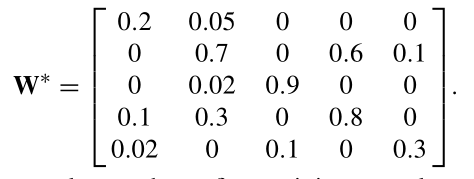
\includegraphics{matrix}	
	于是针对每个样本的合适k值分别为该样本对应的列中非零元素的个数-1。依次为2,3,1,1,1。
	至此稀疏重构阶段已经完成,我们得到了全体训练样本的合适k值,下一步是用全体训练样本及其对应的k值构建kTree。
	\subsection{kTree}
	因为kTree是仿照ID3算法建立的决策树,所以我们先介绍ID3算法。利用决策树进行分类分为两步:首先利用训练样本建立决策树模型,然后利用得到的决策树对测试样本分类。下面介绍ID3算法的建树过程。
	\subsubsection{ID3算法}
	从根结点开始创建决策树,每一个结点都是当前的最优划分属性。ID3算法中选择最优划分属性的准则是信息增益。要理解信息增益,需要从信息熵说起。
	
	信息熵是衡量样本集合纯度(或者说不确定性)的一个指标,设当前样本集合D中第k类样本所占的比例为$ p_k $,则信息熵定义为:
	\begin{equation}
	Ent(D) = -\sum_{k=1}^{\vert y \vert}p_{k}log_{2}p_k
	\end{equation}
	其中$ \vert y \vert $为样本中总类别数。$ Ent(D) $值越小,样本纯度越高。这样定义的原因是:信息熵表示系统的不确定性,是关于事件发生概率的函数。而一件事发生的概率越高,对应的不确定性就越低,因此信息熵首先是概率的减函数;其次,两个独立事件同时发生时对应的不确定性应该等于这两个事件各自发生时的不确定性之和。对数函数加上负号可以满足这两个条件,因此有上式的定义。
	
	在信息熵的基础上,定义某个属性信息增益:当前样本的信息熵-根据该属性划分后所得样本的信息熵。也就是根据该属性的划分对样本纯度的提升程度。于是对信息增益有如下定义:
	\begin{equation}
	Gain(D,a) = Ent(D) - \sum_{v=1}^{V}\frac{\vert D^{v} \vert}{\vert D \vert}Ent(D^v)
	\end{equation}
	在每一步划分时,ID3算法选择信息增益最大的属性作为划分属性,如此递归划分。有三种情况会导致递归返回:
	
	1.当前结点包含的样本属于同一类别,无需划分;
	
	2.当前属性集为空,或所有样本在所有属性上取值相同,无法划分;
	
	2.当前结点包含的样本集合为空,无法划分。
	
	这样最终建成了决策树,决策树的每个叶结点对应样本的一个类别。建树完成之后,在分类阶段,对于每一个测试样本,从根结点开始对照,直到最后被划分至一个叶结点。将叶结点对应的类别作为该测试样本的类别。
	\subsubsection{仿照ID3算法建立kTree}
	我们仿照ID3算法来创建kTree:ID3算法用每个训练样本的类别作为其标签,而kTree用每个训练样本的最优k值作为其标签。{\bfseries 这样做的理论依据是:ID3算法的建树过程中,在各个分支结点上属性相同的训练样本被划分至同一个类别。于是这些样本间的距离应该较小,可以认为它们有相同或相近的k值。}在kTree中,我们认为这些样本有相同的k值。
	
	按上述方法建树之后,k值相同的训练样本被划分到同一个叶结点中。在测试过程中,给出一个测试样本,在kTree中找到它对应的叶结点,就将该叶结点对应的k值作为该测试样本的k值。构建kTree的流程如图所示:
	
	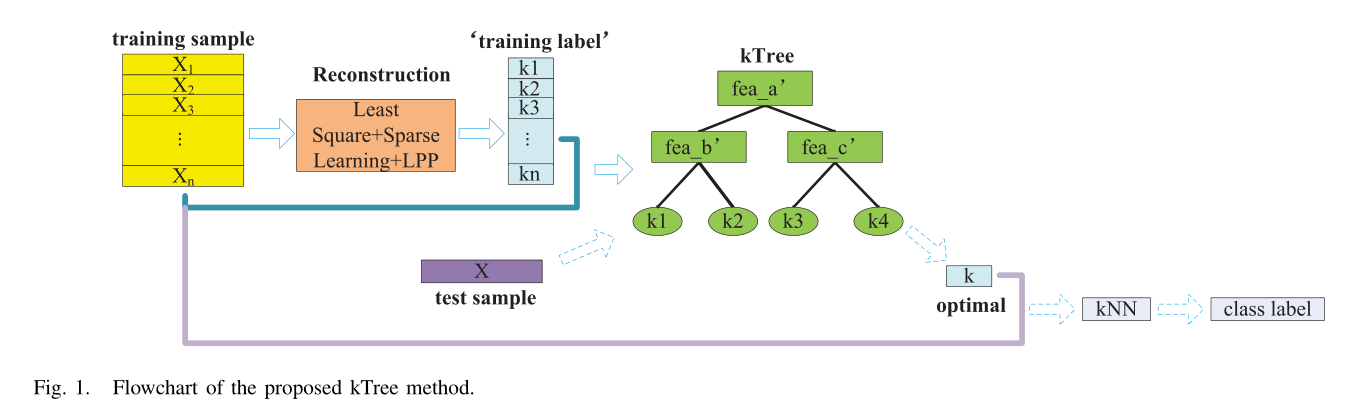
\includegraphics[scale=0.3]{kTree}
	
	下面分析一下kTree方法的时间复杂度。在测试阶段,找到每个样本的k近邻需要$ O(log(d)+ n) $。相比之下,之前基于图稀疏重构的kNN方法需要$ O(n^2) $,固定k值的方法需要$ O(n^{2}d) $。至此第一部分已经完成,{\bfseries 为每个测试样本快速输出了合适的k值}。接下来进一步降低时间复杂度。
	\section{快速找到k近邻}
	\subsection{基于kTree的k*Tree方法}
	kTree方法在得到k值之后,仍然要在全体训练样本中寻找测试样本的k近邻。其实只需要在一部分训练样本中寻找k近邻就足够了。因此对kTree方法作出改进:在叶结点中加入额外的信息,也就是训练样本的一个子集。在得到k值之后,只在这个子集中寻找k近邻。k*Tree的流程如图所示:
	
	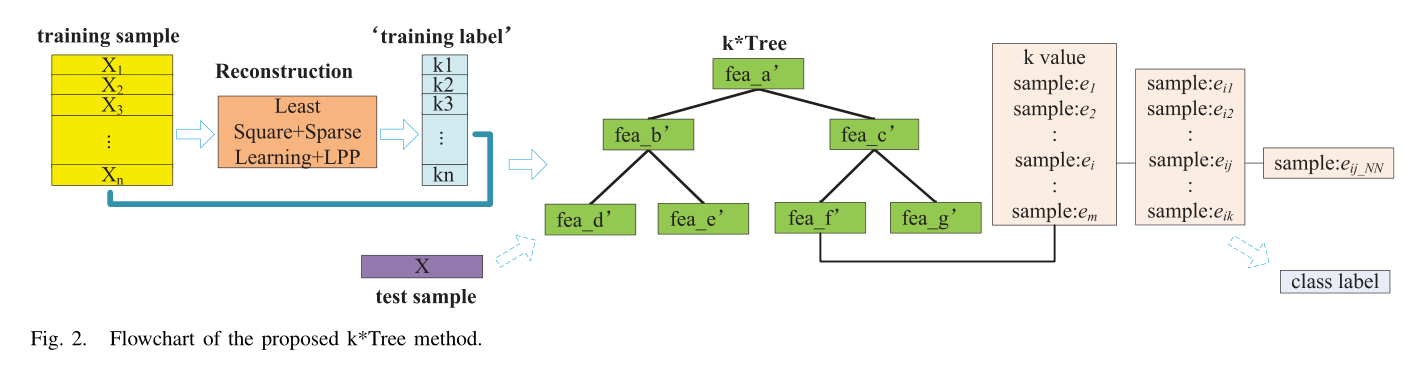
\includegraphics[scale=0.3]{kStarTree}
	
	\section{待改进的地方}
	\subsection{在建树过程中加入启发式信息}
	在ID3算法中,选择最优划分属性的唯一准则是信息增益。因为kTree是仿照ID3算法,它的划分准则也只有信息增益。于是我们设想,在划分准则中加入一些启发式信息,可能会创建出分类效果更好的决策树。
	
	启发式信息是指与问题本身相关的一些先验信息。这些信息对于问题求解有指导或启发作用,因而称为启发式信息。
	
	由于启发式搜索只有有限的信息(比如当前状态的描述),要想预测进一步搜索过程中状态空间的具体行为则很难。一个启发式搜索可能得到一个次最佳解,也可能一无所获。这是启发式搜索固有的局限性。{\bfseries 这种局限性不可能由所谓更好的启发式策略或更有效的搜索算法来消除。}
	
	针对kTree,在每一步划分时可以考虑加入启发式信息,也就是选择新的划分准则,而不是只考虑信息熵。然而有研究表明,划分准则的选取虽然对决策树的尺寸有较大影响,{\bfseries 对泛化性能的影响却很有限。}
	
	这里的启发式信息有待研究。
	\subsection{如何体现所有样本}
	在kTree方法的建树过程中,为了防止过拟合,加入剪枝的步骤。因此不能体现所有样本。
	
	剪枝是为了处理过拟合,因为有时会把训练集自身的一些特点当作所有数据都具有的一般性质。{\bfseries 过度拟合一方面影响决策树的分类精度,另一方面会导致决策树规模过大。}剪枝分为预剪枝和后剪枝:
	
	预剪枝是对每个结点,在划分前先进行估计,若该结点的划分不能带来泛化性能的提升,则停止划分并将该结点标记为叶结点。预剪枝的优点:减少时间开销。缺点:可能导致欠拟合。因为某些分支的当前划分不能带来性能提升,但在其基础上进行的后续划分可能带来性能提升。
	
	后剪枝是先生成一棵完整的决策树,然后自底向上对非叶结点进行考察。若将该结点替换为叶结点能带来泛化性能的提升,则将该结点替换为叶节点。后剪枝的优点:通常比预剪枝保留了更多的分支,泛化性能更好。缺点:时间开销大。
	
	剪枝方法和程度对泛化性能的影响相当显著。研究表明,在数据带有噪声时,通过剪枝最高可将泛化性能提高$ 25\% $。
	
	如何在kTree中体现所有样本,或者用一种新的数据结构来体现所有样本,有待研究。
	
	\begin{thebibliography}{99}
		\bibitem{book1}X. Zhu, Z. Huang, H. T. Shen, and X. Zhao, “Linear cross-modal hashing
		for efficient multimedia search,” in Proc. ACM MM, 2013, pp. 143–152.
		\bibitem{book1}X. Zhu, L. Zhang, and Z. Huang, “A sparse embedding and least variance
		encoding approach to hashing,” IEEE Trans. Image Process., vol. 23,
		no. 9, pp. 3737–3750, Sep. 2014.
		\bibitem{book1}X. Zhu, Z. Huang, Y. Yang, H. T. Shen, C. Xu, and J. Luo, “Self-
		taught dimensionality reduction on the high-dimensional small-sized
		data,” Pattern Recognit., vol. 46, no. 1, pp. 215–229, 2013.
		\bibitem{book1} J. Zhang, M. Wang, S. Zhang, X. Li, and X. Wu, “Spatiochromatic
		context modeling for color saliency analysis,” IEEE Trans. Neural Netw.
		Learn. Syst., vol. 27, no. 6, pp. 1177–1189, Jun. 2016.
		\bibitem{book1}He X, Niyogi P. "Locality preserving projections",Advances in neural information processing systems. 2004: 153-160.
	\end{thebibliography}
\end{document}